\documentclass{article}
\title{iptables case-studies}
\author{Fabio Massimo Ercoli
	\footnote{
		More on me:
		\href{https://github.com/fax4ever}{my GitHub page} -
		\href{https://www.linkedin.com/in/fabioercoli}{my Linkedin page}.
}}
\date{December 28\textsuperscript{th} 2024}
\usepackage{listings}
\usepackage{hyperref}
\usepackage{color, colortbl}
\usepackage{graphicx}
	\graphicspath{ {./images/} }
\usepackage{subfig}	

\begin{document}
\maketitle
\thispagestyle{empty}

\section{Set up Linux Server VM}
To test a firewall what we really need is a server Linux distribution like Fedora server,
that does not have by default a graphic environment, but it is only
accessible by shell (local / remote).

To setup the VM I use \href{https://virt-manager.org/}{Virt Manager} as a virtual environment,
that is based on the KVM virtualization.

These are commands to install and start it: 

\begin{verbatim}
sudo dnf install @virtualization
sudo systemctl start libvirtd
virt-manager
\end{verbatim}

The ISO of the operating system can be downloaded from the
\href{https://fedoraproject.org/server/download}{Fedora Server portal}.
In a few steps we can install our Fedora Server.
We don't need much memory and CPUs, the OS is very lightweight. See figure 1 and 2.

In one of the picture we can see that we keep the default virtual network configuration,
using \emph{NAT}, that is the simplest way of accessing an external network from a virtual machine.
 A virtual machine with NAT enabled acts much like a real computer that connects to the Internet through a router.
 
The \emph{iptable} software is provided by default by the Linux distribution.
Prompting: 

\begin{verbatim}
iptables --version
\end{verbatim}

\noindent We get the version in use:

\begin{verbatim}
iptables v1.8.10 (nf_tables)
\end{verbatim}

\begin{figure}%
	\centering
	\subfloat[\centering Memory CPU]{{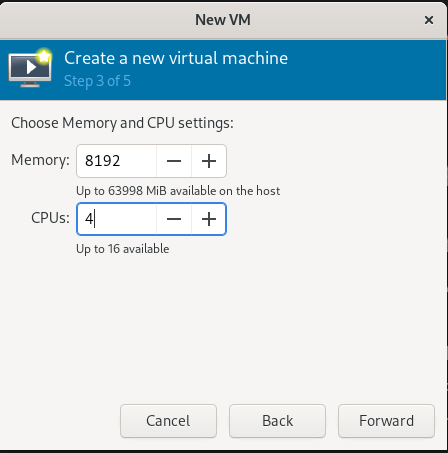
\includegraphics[width=5cm]{h8-1} }}%
	\qquad
	\subfloat[\centering Disk]{{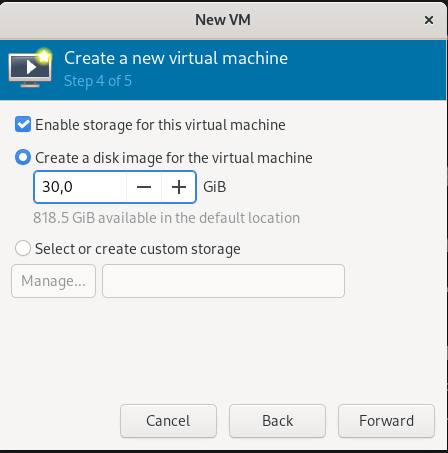
\includegraphics[width=5cm]{h8-2} }}%
	\caption{Linux VM resources}%
	\label{fig:vm-resources}%
\end{figure}

\begin{figure}%
	\centering
	\subfloat[\centering Network]{{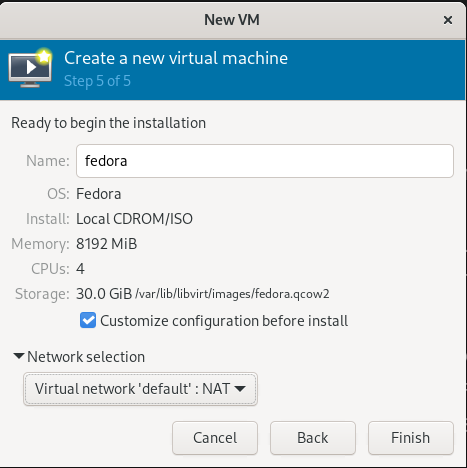
\includegraphics[width=5cm]{h8-3} }}%
	\qquad
	\subfloat[\centering Installation settings]{{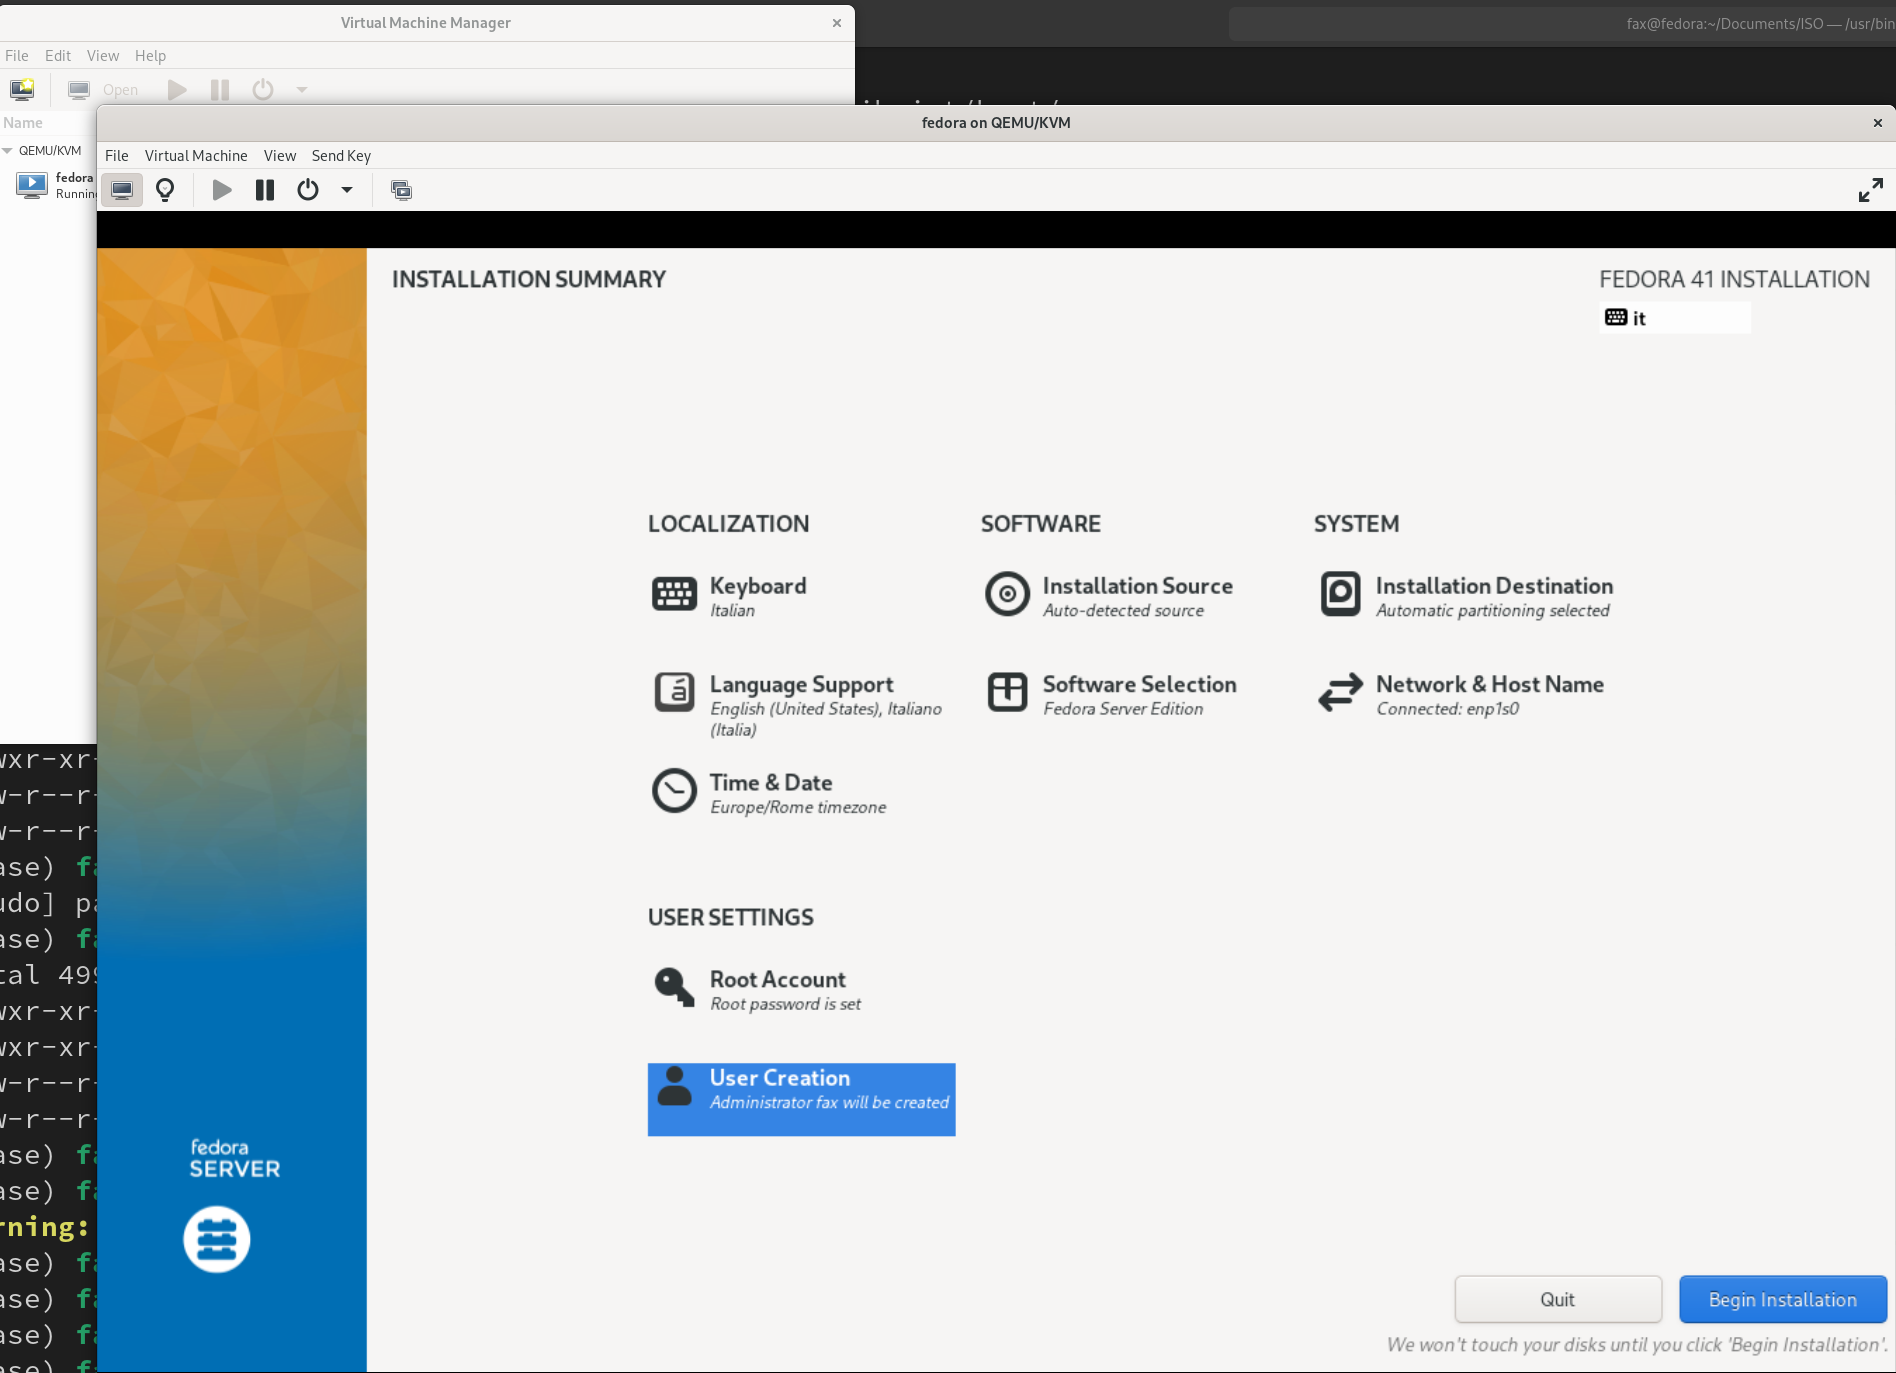
\includegraphics[width=5cm]{h8-4} }}%
	\caption{Configure Linux VM}%
	\label{fig:va-settings}%
\end{figure}

\section{Scenario: Allow the guest VM to access the internet}

\subsection{Information security requirements}

The \emph{guest} VM we have just created does not have any access to the external internet.
With the NAT configuration all the traffic incoming to and outgoing from
the \emph{guest} VM
is supposed to pass through the \emph{host} operating system.
The host operating system is another Fedora Linux, this time a workstation edition
and probably it does not allow by default the traffic to pass through it.

We want to allow any connection from/to the external internet
to pass through the \emph{host} operating system
in order to make the \emph{guest} VM connected.

\subsection{Test before the configuration}

To test the fact that the VM is isolated from the external internet,
we can try the following \emph{wget} command:

\begin{verbatim}
wget www.facebook.com 
\end{verbatim}

This command blocks without returning  if it is run from the \emph{guest} VM
console, while it works perfectly if it is run from the \emph{host} OS.

\subsection{Configure iptables to meet the requirements}

In this case we need to verify the iptables configuration of the
\emph{host} operating system, in particular looking at the \emph{filter} table,
chain \emph{FORWARD}.

To inspect all the chains of the filter table.
We can run the command:

\begin{verbatim}
sudo iptables -vL
\end{verbatim}

We can immediately notice that the default policy of the \emph{FORWARD} is \emph{DROP}. 
Furthermore, since we called the command with the \emph{v} verbose option,
we notice that some packets have been blocked:

\begin{verbatim}
Chain FORWARD (policy DROP 175 packets, 15712 bytes)
\end{verbatim}

Inspecting the network we get the \emph{guest} VM
IP address, that in this case is \emph{192.168.124.203}.
This address is a virtual address managed by the virtual network
defined on the \emph{host} machine.
We can add a rule on top of the chain:

\begin{verbatim}
sudo iptables -I FORWARD -d 192.168.124.203 -j ACCEPT
sudo iptables -I FORWARD -s 192.168.124.203 -j ACCEPT
\end{verbatim}

And verifying that is has been acquired:

\begin{verbatim}
Chain FORWARD (policy DROP 175 packets, 15712 bytes)
pkts bytes target     prot opt in     out     source               destination         
0    0 	   ACCEPT     all  --  any    any     192.168.124.203      anywhere            
0    0     ACCEPT     all  --  any    any     anywhere             192.168.124.203 
\end{verbatim}

\subsection{Test after the configuration}

Redoing the same \emph{wget} on the guest VM, we can now
access to the \emph{www.facebook.com} URL:

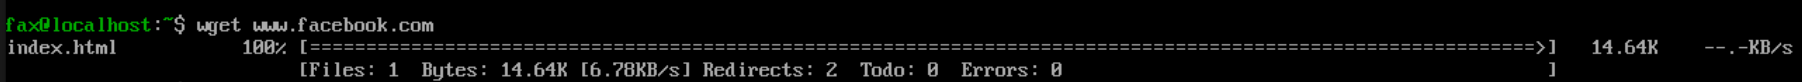
\includegraphics[width=13cm]{h8-5}

\noindent Moreover can query again the \emph{iptable} on the host machine and see:

\begin{verbatim}
Chain FORWARD (policy DROP 175 packets, 15712 bytes)
pkts bytes target     prot opt in     out     source            destination         
595  37000 ACCEPT     all  --  any    any     192.168.124.203   anywhere            
1079 1572K ACCEPT     all  --  any    any     anywhere          192.168.124.203  
\end{verbatim}

That some packets have been passed though the host machine
matching the rules we have just defined.

Another nice thing that we can notice it that we didn't need to restart the \emph{iptables}
nor the \emph{virt-manager} demons.
The changes have been applied on the fly!

\section{Scenario : prevent users to use a given portal}

\subsection{Information security requirements}

We don't want people using VM can access to the \emph{www.facebook.com}
portal. We want to limit the distractions of our employees.
We already tested that it is now possible to access the portal.

\subsection{Configure iptables to meet the requirements}

One option would be configure \emph{FORWARD} chain on
the \emph{host} operating filter, another option would be to
configure \emph{iptables} on the \emph{guest} VM.

I'll follow this second option.

Querying \emph{iptables} of the \emph{guest} VM,
we can see here that the chains of the filter tables are all empty
and have all \emph{ACCEPT} as default policy.

We can create a \emph{sh} script like the following one:

\begin{lstlisting}[language=bash]
#!/bin/bash
for blockip in `resolveip facebook.com | cut -d "  " -f 6`; do
 sudo iptables -A OUTPUT -o eth0 -p tcp -d $blockip -j DROP
 sudo iptables -A INPUT -p tcp -s $blockip -j DROP
done
\end{lstlisting}

a couple of rules are added for each IP address to block.
Running the script should add the rules on the \emph{host} VM.
Notice that \emph{resolveip}, if not present, is supposed to be installed using the command:

\begin{lstlisting}[language=bash]
	sudo dnf install resolveip
\end{lstlisting}

\subsection{Test after the configuration}

Again, without the need of restarting the \emph{ipconfig} service,
we can check that now the command does not work anymore,
and one of the blocking rule we've defined has matched some packets.

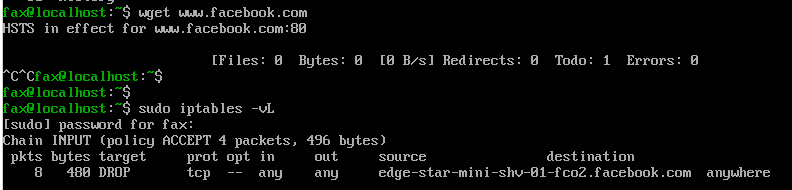
\includegraphics[width=13cm]{h8-6}

To check that this configuration does not affect the use of other
sites , such as \emph{redhat.com}, trying a:

\begin{verbatim}
	wget www.redhat.dom
\end{verbatim}

\noindent the packets are not blocked in this case:

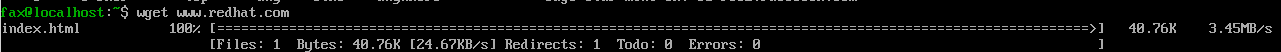
\includegraphics[width=13cm]{h8-7}

\section{Scenario: limiting the access to an HTTP server}

\subsection{Information security requirements}

In our guest machine we're going to install an instance of 
\href{https://httpd.apache.org/}{Apache HTTPd server}.
We want to demonstrate how to forbid the use of the service from
the host machine.

This is an example of limiting the access to the server.

Moreover, we want to extract the rules we need to define for this scenario 
in a different (user-defined) chain, so that they can be potentially reused.

 \subsection{Install the Apache service}
 
To install the Apache server on the VM machine we can run the following commands: 
 
\begin{lstlisting}[language=bash]
sudo dnf install httpd -y
sudo systemctl start httpd.service
sudo firewall-cmd --add-service=http
\end{lstlisting}

The first command install the binary on the filesystem,
the second one starts the process as service OS (daemon),
the last command allows to receive connections from outside
on the port 80, using this time OS firewall.
That is probably an application level firewall, since it
has the concept of application level protocol (http in this case).

\subsection{Test before the configuration}

The Apache HTTP hello page is accessible from the browser
running from the host machine:

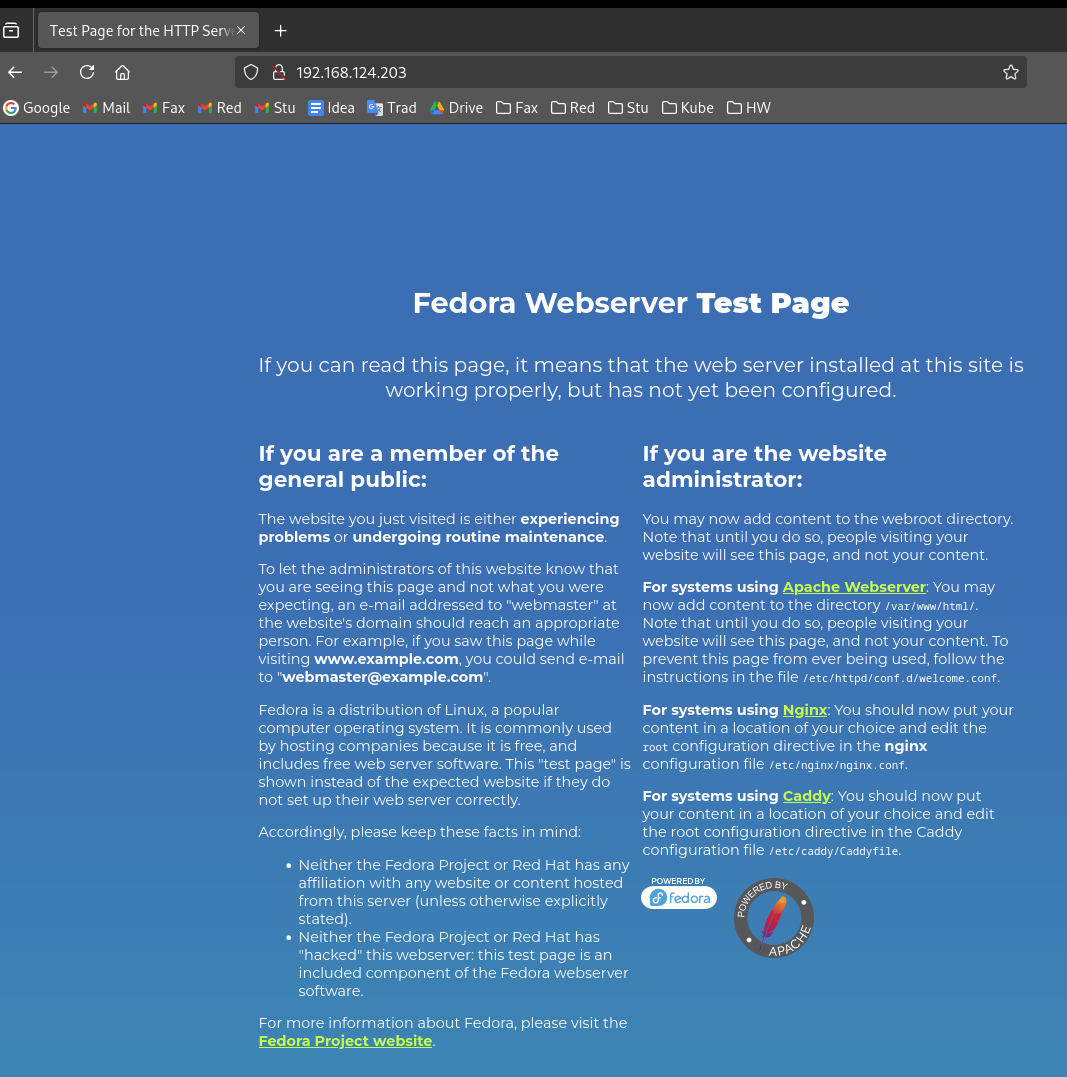
\includegraphics[width=13cm]{h8-8}

\subsection{Configure iptables to meet the requirements}

We can have the IP address of the host machine looking at
the Apache access logs:

\begin{lstlisting}[language=bash]
sudo cat /var/log/httpd/access_log
\end{lstlisting}

The host machine seen from the guest machine has IP address: \emph{192.168.124.1}.

I create two custom chains on the default IP table, filtering:
\emph{input-apache-chain}, \emph{output-apache-chain}, 
deleting also possible pre-existing custom chains and associations:

\begin{lstlisting}[language=bash]
sudo iptables -F
sudo iptables -X
sudo iptables -N input-apache-chain
sudo iptables -A input-apache-chain -p tcp -m multiport --dports 80,443 
  -s 192.168.124.1 -m state --state NEW,ESTABLISHED,RELATED -j DROP
sudo iptables -A INPUT -j input-apache-chain
sudo iptables -N output-apache-chain
sudo iptables -A output-apache-chain -p tcp -m multiport --sports 80,443 
  -d 192.168.124.1 -m state --state NEW,ESTABLISHED,RELATED -j DROP
sudo iptables -A OUTPUT -j output-apache-chain
\end{lstlisting}

\noindent Executing the \emph{sudo iptables -vL} we get:

\begin{verbatim}
Chain INPUT (policy ACCEPT 374 packets, 32712 bytes)
pkts bytes target     		  prot opt in     out     source     destination         
388  33552 input-apache-chain all  --  any    any     anywhere   anywhere            

Chain OUTPUT (policy ACCEPT 102 packets, 9168 bytes)
pkts bytes target     		   prot opt in     out     source    destination         
102  9168  output-apache-chain all  --  any    any     anywhere  anywhere            

Chain input-apache-chain (1 references)
pkts bytes target     prot opt in     out     source         destination         
14   840   DROP       tcp  --  any    any     _gateway       anywhere             
multiport dports http,https state NEW,RELATED,ESTABLISHED

Chain output-apache-chain (1 references)
pkts bytes target     prot opt in     out     source         destination         
0    0     DROP       tcp  --  any    any     anywhere       _gateway             
multiport sports http,https state NEW,RELATED,ESTABLISHED
\end{verbatim}

\subsection{Test after the configuration}

Immediately after applying the rule the Apache hello page became no longer
callable from the Firefox run from the \emph{host} machine, as desired.

\section{Persist and reload the iptables configuration}

Any change to the \emph{iptables} configuration is lost,
when the operating system is restated.

The current configuration can be serialized to some file using \emph{iptables-save}:
\begin{lstlisting}[language=bash]
 sudo iptables-save > my-iptables
\end{lstlisting}

When the system is restarted, the configuration can be reloaded using \emph{iptables-restore}:
\begin{lstlisting}[language=bash]
 sudo iptables-restore > my-iptables
\end{lstlisting}

The load can be automatized adding the latter command
to some script that we know it is always run at startup.
For instance \emph{.bash\_profile} or \emph{.bashrc}.
System administrators know that.

\section{Extra: use SSH to configure the VM}

Instead of using the bash provided directly by the virtual environment,
we can use \emph{SSH} to run commands on the remote \emph{guest} VM
operating system directly using the shell of the \emph{host} machine.

We can connect to the VM \emph{guest} OS, just typing:
\begin{verbatim}
	ssh 192.168.124.203
\end{verbatim}

In this case the username \emph{fax} is the name of both the client and server,
so it does not need to be retyped.
Password is required.
This can be avoided using client certificates, they also improve the security and efficiency...
	
\end{document}	